%===========================
\chapter{Project Evaluation}
%===========================
This chapter gives an evaluation of the project and the course, TDT4290 Customer Driven Project. The main focus is to describe the how the team evolved and how work was done during the project.   

%----------------------------------
\section{Team Dynamics}
%----------------------------------
The forming and development of the team are described in this section.
%----------------------------------
\subsection{Goals and Team Building}
%----------------------------------
The project started out with randomly assigned student groups of six to seven people. This was done intentionally to learn the students to work in a realistic setting. Our group consisted of six Norwegian students and one Czech student. 

As one of the team members was a foreign student, all the internal team communication had to be done in english. In addition our advisors were english speaking, so the whole project was done in english. This did not occur as a problem, because all the team members both spoke and wrote english fluently.

At the first meeting we decided to state our personal goals for the project. This resulted in the following list:
\begin{itemize}
	\item Improve programming skills.
	\item Learn to develop software efficiently.
	\item Learn to work in a realistic environment.
	\item Fulfill the needs of the customer. 
\end{itemize}
These goals match the course's goals, with some extensions. All these goals was common for the team members, which resulted in good cooperation from the start and an agreement of what we wanted to achieve in the project. The decision to characterize ourselves as a team came early in the project, which is defined to be a collection of people working interdependently and is committed to achieve one common goal.

None of the team members had any relations with each other when the project started. During the project we learned how to work together in a professionally and efficient manner. Getting there was a demanding task and is described more thoroughly in the section regarding team evolution.

\subsection{Team Evolution}
%---------------------------------
During the first weeks of the project the team were in a good, but also uncertain stage. The team members did not know the boundaries of the others and tried to not end up in an argument. This resulted in a series of matters; responsibility for tasks were not taken and no one dared to ask why tasks was not done.

The team realized the problems.

\section{Risk Handling}
%----------------------------------
Some of the risks predicted in the planning phase occured to a certain degree during the project.
This section will discuss those risks and how they were handled.

\paragraph{R4. Illness/Absence}
In general, not many team members were absent for longer periods.
One team member was away in northern Norway for a week on vacation, and another was sick for a week and a half. This caused some delay on a few tasks, as the absentees had to get up to date on the state of the project, but it did not majorly hinder the progress of the team. The consequence of this risk was also diminished by the fact that it occured early in the project, and that the team members who were absent did not work on critical tasks at the time.

\paragraph{R6. Conflicts within team}
In the start of the project, the team members were divided on which tools to use, and on which programming language to use. Because of this, the team had to spend some time discussing back and forth. After some constructive discussions the team was able to come to a mutual decision.

Also, some team members felt that it was not realistic that the course should demand 25 hours from each member. As the project progressed, it quickly became apparent that this number of hours were needed to complete the project in a satisfying manner. This led to an overall increase in work effort in the team.

\paragraph{R8. Miscommunication within team}
During sprint 3, the ones responsible for creating test data and the ones writing the test cases did not clearly communicate with each other. This led to having to make small changes in some of the test cases to be able to use the test data.

The test responsible wrote test cases for functionality that the programming team had not thought about. For example, checking that you are not allowed two platforms with the same platform ID.
When the problem was detected, all essential functionality was added.

\paragraph{R10. Lack of experience with Scrum}
As the team had no previous experience with Scrum, the project got off to a slow start.
After evaluating the first sprint, it quickly became apparent that the process was far from perfect.
The second sprint was an improvement of the first, and the planning meeting was longer and more detailed, but in our opinion it was still not good enough. We felt that we did not adhere to proper Scrum, and that we did not properly explain the different tasks in the backlog. In the last two sprints, we felt that we had achieved a better understanding, and this really showed in the process. A more detailed discussion can be found in the Scrum section.

\paragraph{R11. Requirements added or modified late in the project}
At the customer meeting on the first day of sprint 4, the customer suggested several new requirements that they would like is to implement. Some requirements were also modified, as we had not implemented them exactly the way they wanted us to.

As we had to focus on tweaking some functionalities to work on their code, and also had to spend time on writing the report, we had to tell the customer that we would probably not be able to finish all the new requirements. This is because implementing a requirement would also require testing, user documentation and additional report work, which is something we could not afford to allot time for.


%--------------------------------
\section{The Process}
%under construction!
%--------------------------------
TODO: Sondre

%-----------------
\subsection{Scrum}
%-----------------
During the preliminary study, we decided to use an agile development method, 
to be able to adopt to changes in requirement during the project, so we 
decided to use Scrum. None of the team member had any previous experience with 
Scrum. In the beginning of the course we had a lecture about Scrum, and we 
got a basic insight in how Scrum works.

When the first sprint planning was finished, we understood that we did not 
follow Scrum properly. The meeting was very short, and we did not do any 
design during the sprint planning. The work items from the sprint was wrong 
estimated, and was not divided propely into work items. For each sprints we 
improved, and the scrum process was good in the end of the project.

Some of team members feel that we followed Scrum to strict, instead of doing 
what that was best for the project. In the end of the project we needed to use 
much time on fixing the utility so it run on the customer's code, since we 
could not change our sprint plan, we ended up with a very high workload.

During the project we learned the advantages of using Scrum, since we could 
get some feedback on the work we had done from the customer, and then improve 
the features to what the customer exactly wanted. 

%------------------------
\section{Time Estimation}
%------------------------
In total there was estimated a total of 2275 hours for this project. We put a 
little more effort in this project and ended up on 2331 hours. This mean we 
was a little over the estimate, and the reason mainly because we wanted to the 
utility work for the customer and a decent amount of work on the report in the 
end of the project. 

The work breakdown structures in \autoref{tab:wbs}, shows the estimated and 
actual hours for each task. The estimates are quite good on most of the task, 
for project management we have used 454 hours, and 275 hours was estimated. 
The reason that we used so many houes on project management is that we had 
weekly meeting with both customer and advisor. In addition to this we had 
internal meetings in the team, and all daily Scrum meeting was registered as 
Project Management. In the start of the project some of the effort was 
registered, so the amount of time spent on project managemnt is actual lower.

In each of the sprints we estimated time for the work items. The estimation 
was based on that every team member should be able to finish the task on the 
estimated time. So in total the work items was overestimated, because some 
team members had more experience, and could finish the task much faster.

The time distribution by task is shown in \autoref{fig:time_by_task}. Nearly 
20\% of the time was used on the project management, for the planning, 
preliminary studies and requirement specificaiton was approximate 10\%, 
actually is this higher, because of some wrong registration of effort in the 
start of the project. The total time that was used for the sprints was over 
40\%., which is a good amount for the development of CSjark. 

\begin{figure}[htb]
	\center
	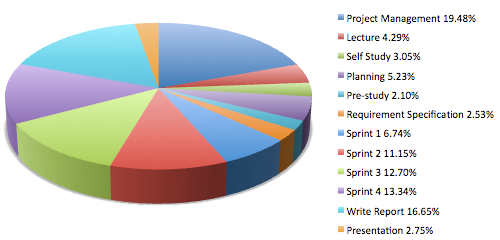
\includegraphics[width=\textwidth]{./evaluation/img/piechart_time}
	\caption{Time Distribution by Task\label{fig:time_by_task}}
\end{figure}

In the start of the project there was low activity, but effort per week 
increased during the project. Effort registered per week can be seen in 
\autoref{fig:time_by_week}. To achieve the 2275 hours in total for the 
project, 175 hours per week was needed. The effort in week 12 was high because 
we needed to finish the last sprint and very much work on the report was done.

\begin{figure}[htb]
	\center
	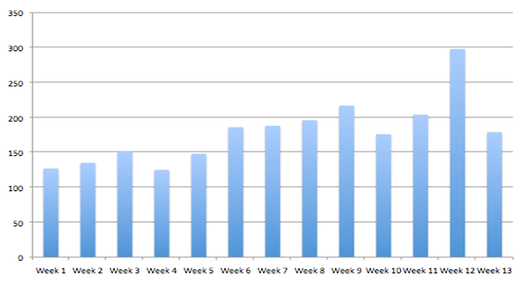
\includegraphics[width=\textwidth]{./evaluation/img/columnchart_effort} 
	\caption{Time Distribution by Week\label{fig:time_by_week}}
\end{figure}

%-------------------------------
\section{Quality Assurance}
%-------------------------------
At the start of the project we made several plans for ensuring quality of the project. This section discusses which of those plans did not work out and what we ended up doing instead.

Initially we planned that we would have peer review of all of the code written for the utility. This plan was something that we were unable to follow up on, mostly due to the poor planning meetings in sprint one and two where the time needed for pair review was not taken into consideration. This made it difficult to organize who was going to do the peer reviews and how we were supposed to find the time to do them. In the end, the lead programmer ended up reviewing most of the code written by the other developers, but the group consensus was that the quality of the code was good enough that it would have been irresponsible to spend more time on peer reviews.

During every sprint the team was supposed to provide the advisor with up to date information regarding the report and the progress with the utility. This was not followed up on as the team members did not want to submit unfinished work to the advisor. This proved to be a problem towards the end of the project forcing the team to start submitting more of the report work to the advisor. As this was not done earlier in the project, the team instead had to organize for several of the members to go through the early stages of the report and raise the quality of the documents internally.

It was planned that the team member responsible for the document was supposed to keep a bird's eye view of the report and go through the different entries before the end of each sprint. This proved to be too much work for just one person. We therefore also made sure that in several other team members would support the one responsible for having a proper overview of the report 

%----------------
\section{Customer Relations}
%----------------
Our relationship with the customer was good throughout the entire project.
We were assigned two customer representatives. As they were developers themselves, they both had a technical background. This made it easier to communicate with the customer.
They knew exactly what they wanted, and were more than happy to give feedback and tips on the implementation of the different requirements. When we first received the initial requirements, we did not fully understand them. After some meetings and dicussions, both internally and with the customer, the team was able to provide the customer with a clear requirement specification that they accepted.

One of the customer contacts was a member of Wireshark's core development team. When we discovered bugs in Wireshark, he could fix them and apply a patch. He also had insight into how 
Lua dissectors were built, and how they interacted with Wireshark. This was a major asset to the team. When we encountered problems during implementation, the customer was able to give us invaluable feedback on how to proceed. This is something that a less technical customer would not have been able to give us.

Each week we had a meeting with the customer where we demonstrated the requirements we had implemented since last meeting. The customer then gave us feedback on the functionalities, and told us what we had to change or improve. This way, any misunderstandings were detected and dealt with in a swift manner.

The customer contacts also had access to our repository, thus they could test the utility themselves.
This meant that they could get a first hand-experience of the utility, and could more easily detect bugs and other issues.	

A problem we had was that, due to security issues, Thales could not allow us to test our utility on their source code. This meant that we had to do some guessing during the implementation, and getting the utility to work on their code was a difficult process. Luckily, Thales gave us the opportunity to send two of our members to them for a few days, as documented in the test section of sprint 4. That gave us an opportunity to fix most of the bugs that we encountered, and in the end the customer said that they were happy with our utility. They approved all the requirements we had listed, although a few of the optional requirements were not implemented due to time constraints.
Overall the customer felt that we were flexible, and adhered to most of their needs.

The week before the end of the project, the team had a presentation at Thales for our advisor, the customer contacts, and some other employees of Thales. The employees that were there are probable users of the dissectors that our utility creates. Due to this, the presentation was focused on the demonstration of the utility, where we showed how the structs were dissected in Wireshark.

The customer also got one of their co-workers to read CSjark's user manual.
The user manual was a little too unclear in some parts, so we used that feedback to improve it, and increase its quality.

The team felt that we were lucky with the customer that we were assigned.
The fact that they knew exactly what they wanted, had a technical background and showed great enthusiasm for the project, made the project more manageable. This also increased the motivation for the team. We felt that they were interested in what we were developing, which ensured a good meeting atmosphere and a good working relationship. Throughout the entire project, they gave us essential feedback on the implementation and requirements, and they were not afraid to tell us if we did something that they disagreed with. The fact that we had two customer contacts, instead of one, increased the amount of feedback we received, and also meant that there was always one person available for us to contact. All in all, we could not be more satisfied with our customer.


%----------------
\section{Summary}
%----------------
Seven people with different personalities and skillsets were randomly assigned to a group. We received a task that we initially did not quite understand the scope off.
But through hard work, and help and feedback from the advisors and the customer, we managed to create a utility that we are proud of. In the beginning, the process did not go as smoothly as we wanted it to, as we struggled to fully grasp and utilize Scrum. After a few sprints, we felt that we understood more, and this led to an increase in both work effort and cooperation. People took more responsibility, and we started to feel like a team with a common goal. We ended up with a utility that fully covered the initial requirements, and a solution that both us and the customer are satisfied with. To summarize, this has been a challenging project, but also a great learning experience.


